% 与英文共用 BASE2/SCALE0 逐种子成功次数。
\begin{figure*}[t]
\centering
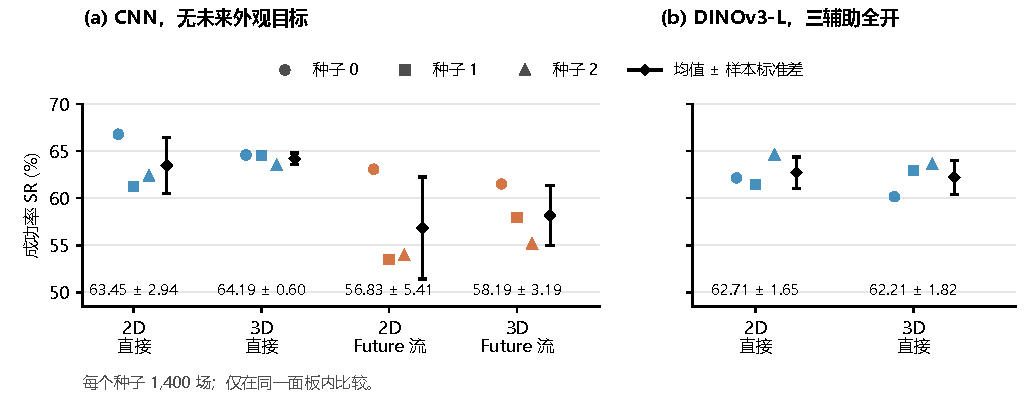
\includegraphics[width=\textwidth]{design_studies/prediction_path_zh.pdf}
\caption{\textbf{表示与预测路径。}彩色标记表示三个训练种子，每个种子评测 1{,}400 个开发场景；黑色菱形及误差线表示均值与样本标准差，下方同时列出数值。两面板均保留 SE(3) 与当前目标 RGB 监督。
(a) CNN，无未来外观目标：直接回归与 Future 流的流匹配配方。
(b) 冻结 DINOv3-L、直接回归、三项外观目标全开。仅在面板内比较；种子间离散程度不是置信区间。}
\label{fig:prediction_path}
\end{figure*}
